\setlength{\parindent}{0ex}
\subsection{Movimiento}
En este apartado veremos un repaso de los movimientos más básicos.


\subsubsection{MRU y MRUA}

Partiendo de la \textit{\(2^a\) Ley de Newton}, sabemos que la Fuerza es igual a la masa por su aceleración:
\[\vec{F} = m\vec{a}\]
Podemos descomponer la fuerza en sus componentes horizontales y verticales:
\[
        \vec{F_{x}}=\frac{\partial^{2}\vec{x}}{\partial{t}}m
        \to
        m\frac{\partial^2 \vec{x}}{\partial t} = 0
        \Leftrightarrow
        \frac{\partial^2{\vec{x}}}{\partial{t}} = 0
\]
\[
        \vec{F_{y}}=F_{y}\hat{\jmath}
        \to
        \vec{F_y} = m\frac{\partial\vec{v}}{\partial t}\Leftrightarrow
        \frac{\vec{F_y}}{m} = \vec{a_y}
\]
Es decir, cuando \(\vec{F_x}\) = 0N, \(\vec{a}=0\)m/\(s^2\), por lo que la velocidad es constante, \(\vec{v}=cte\), solo si \(\vec{F_y}\neq 0\)N y \(\vec{a_y} = \vec{a} = \frac{\vec{F_y}}{m}=cte\).\par \vspace{0.5cm} Sabiendo esto y las expresiones de la aceleración y la velocidad, podemos definir las expresiones del \textbf{MRU} y \textbf{MRUA}: \par \vspace{0.5cm} \hspace{5cm}
\( \vec{a} = \frac{\partial \vec{v} }{\partial t}\) Y \( \vec{v} = \frac{\partial \vec{x} }{\partial t}\) \par \vspace{0.5cm} Obtenemos:
\[
        \int_{0}^{t}{\vec{a}\hspace{1mm}\partial{t}} = \int_{0}\partial{t}
        \to
        \boxed{\vec{v} = \vec{v_o} + \vec{a}t}
\]
\[
        \int_{0}^{t}{\vec{v}\hspace{1mm}\partial{t}} = \int_{0}{\partial{\vec{x}}}
        \to
        \boxed{\vec{x} = \vec{x_o} + \vec{v_0}t}
\]
\hspace{1.1cm} Si \( \vec{v} = \vec{v_o} + \vec{a}t\)
y
\( \vec{a} = cte \to\) \fbox{\(\vec{x} = \vec{x_o} + \vec{v_0}t + \frac{\vec{a}t^2}{2}\)}

\subsubsection{MCU y MCUA}
\vspace{0.5cm}
\hspace{0.5cm}
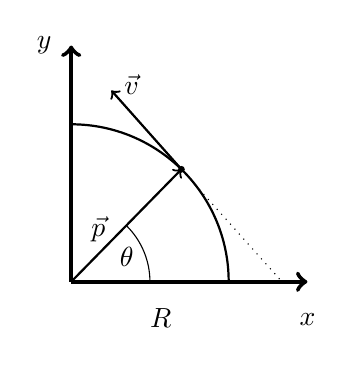
\begin{tikzpicture}[x=1cm,y=1cm]
        \draw[->,ultra thick] (0,0)--(3,0) node[above = -20]{\(x\)} node[above = -13, left = 45] {\(R\)};
        \draw[->,ultra thick] (0,0)--(0,3) node[left = 3]{\(y\)};
        \draw[thick] (2,0) arc (0:90:2);
        \draw[thin] (1,0) arc (0:45:1) node[above = -18]{\( \theta\)};
        \draw[->,thick] (1.4,1.42828) -- (0.5098765432099,2.429629629629) node[above = 2, right = 1]{\(\vec{v}\)};
        \draw[dotted] (1.4,1.42828) -- (2.676296,0);
        \draw[->,thick] (0,0) -- (1.4,1.42828) node[left = 30, above = -30]{\(\vec{p}\)};
        \filldraw[color = black] (1.4,1.42828) circle (1pt);
\end{tikzpicture}
% TODO ARREGLAR LA FIGURA CORRESPONDIENTE

El \textbf{MCU} o Movimiento Circular Uniforme, se genera en las rotaciones de un cuerpo respecto a un punto \(p\)